\documentclass[journal]{IEEEtran}

\usepackage{cite}
\usepackage{amsmath,amssymb,amsfonts}
\usepackage{algorithm}
\usepackage{algorithmic}
\usepackage{graphicx}
\usepackage{textcomp}
\usepackage{xcolor}
\usepackage{booktabs}
\usepackage{url}
\def\UrlBreaks{\do\/\do-}
\usepackage{microtype}
\usepackage{enumitem}
\usepackage[
  pdftitle={DualTrust: An Ultra-Low-Latency Asymmetric Bayesian Governance Framework for Resilient Autonomous Agent Containment in Cyber-Physical Systems},
  pdfauthor={Khairan Noor Fadhlillah},
  pdfsubject={Autonomous Agents, Multi-Agent Governance, Bayesian Trust Systems, Cyber-Physical Systems},
  pdfkeywords={Autonomous Agents, Multi-Agent Governance, Bayesian Trust Systems, Cyber-Physical Systems, Runtime Verification, Salami-Slicing Resistance, Merkle Audit Trails, Zero-Trust Architecture},
  pdfcreator={pdfLaTeX with IEEEtran},
  colorlinks=false,
  hidelinks
]{hyperref}

\newtheorem{theorem}{Theorem}
\newtheorem{lemma}{Lemma}
\newtheorem{proposition}{Proposition}
\newtheorem{definition}{Definition}
\newtheorem{invariant}{Security Invariant}

\emergencystretch=1.5em

\hyphenation{op-tical net-works semi-conduc-tor}

\begin{document}
\flushbottom

\title{DualTrust: An Ultra-Low-Latency Asymmetric Bayesian Governance Framework for Resilient Autonomous Agent Containment in Cyber-Physical Systems}

\author{Khairan~Noor~Fadhlillah%
\thanks{K. N. Fadhlillah is with the Department of Computer Science, Universitas Ary Ginanjar, Jakarta 12560, Indonesia (e-mail: dev@khairan.tech).}%
\thanks{Manuscript submitted October 27, 2026 for review. Complete source code, automated test harnesses, and microsecond benchmark suites are publicly archived at: \url{https://github.com/codesbykhairannoor/dual-trust}. DualTrust is distributed via PyPI at: \url{https://pypi.org/project/dualtrust/}.}%
}

\markboth{IEEE Transactions on Dependable and Secure Computing,~Vol.~XX, No.~XX, 2026}%
{Fadhlillah: DualTrust: Ultra-Low-Latency Asymmetric Bayesian Governance}

\maketitle

\begin{abstract}
The proliferation of Ambient Wearable Intelligence (AWI) ecosystems---spanning augmented reality glasses, smartwatches, and pervasive edge IoT actuators---is fundamentally transitioning human-AI interaction from explicit tactile commands to continuous, implicit background tool delegation. In these ambient environments, autonomous Large Language Model (LLM) agents are granted operational authority to invoke external APIs, reserve financial micro-quotas, and control physical actuators. However, existing safety guardrails depend on secondary LLM-as-a-judge classifiers that introduce prohibitive runtime latencies (400--850\,ms) and recurring token expenses, while static role-based access control fails against continuous behavioral drift, memory backdoors, and interleaved salami-slicing exploits. We present \textbf{DualTrust}, an ultra-low-latency asymmetric Bayesian governance framework engineered specifically for autonomous multi-agent cyber-physical containment. DualTrust enforces a decoupled principal-agent architecture that strictly isolates Human Principal Accountable Credit from Bayesian Agent Operational Standing. Agent behavior is continuously modulated via an asymmetric power-law slashing engine ($\Delta\beta \propto (\text{sev} \cdot c^2) \cdot v^{1.8}$) with instantaneous clean-streak reset, deterministic SHA-256 64-bucket striped concurrency locks, atomically locked rollback refunds, and an $O(1)$ RAM sliding-window RFC~6962 Merkle audit ledger with rolling epoch seals. Evaluated across 176 automated invariant tests and 10,000-cycle Monte Carlo attack simulations, DualTrust makes deterministic authorization verdicts in a median latency of \textbf{47.10\,$\mu$s} in-memory (mean 63.16\,$\mu$s, tail p99 287.10\,$\mu$s) and \textbf{155.80\,$\mu$s} under persistent SQLite WAL disk transactions, with end-to-end Python decorator wrappers executing in median 60.70\,$\mu$s (async) and 88.30\,$\mu$s (sync) with zero API overhead. Compared against state-of-the-art LLM guardrails, DualTrust achieves over \textbf{6,600$\times$} lower mean latency (up to \textbf{18,000$\times$} lower median latency) and over \textbf{32$\times$} (decorator wrapper) to \textbf{60$\times$} (RAM core) lower latency than localized AST validators, demonstrates Sybil defamation immunity against collusive probation swarms by policy construction, and provides tamper-evident, append-only audit durability with RFC~6962 inclusion verification, establishing a practical, foundational governance runtime for trustworthy ambient intelligence.
\end{abstract}

\begin{IEEEkeywords}
Autonomous Agents, Multi-Agent Governance, Bayesian Trust Systems, Cyber-Physical Systems, Runtime Verification, Salami-Slicing Resistance, Merkle Audit Trails, Zero-Trust Architecture.
\end{IEEEkeywords}

\IEEEpeerreviewmaketitle

\vfill\newpage

\section{Introduction}
\label{sec:intro}

\IEEEPARstart{D}{istributed} computing systems are undergoing a fundamental paradigm transition in human-computer interaction: the shift from handheld screen-mediated interfaces toward \emph{Ambient Wearable Intelligence} (AWI) ecosystems~\cite{sun2026survey}. In this emerging paradigm, physical smartphones are progressively superseded by pervasive edge devices---including smart augmented reality (AR) spectacles, biometric smartwatches, and spatial acoustic nodes~\cite{wu2023autogen}. Within these environments, users no longer navigate application menus or manually confirm transactions. Instead, human principals express declarative, high-level intents verbally or biometrically (e.g., ``secure my daily commute'', ``procure localized computing resources'', ``balance my micro-utility quotas'')~\cite{qin2024toolllm}. 

To fulfill these continuous requests, personal autonomous software agents powered by Large Language Models (LLMs) operate as background proxies. These agents are granted runtime delegation to dynamically discover tools, negotiate with machine-to-machine (M2M) service endpoints, query distributed databases, and execute programmatic side-effects across physical and digital infrastructures~\cite{liu2024agentbench}.

\subsection{The Fundamental Vulnerability of Autonomous Delegation}
While autonomous agent delegation promises unprecedented operational efficiency, it introduces critical cybersecurity and reliability challenges into cyber-physical systems (CPS)~\cite{ruan2024identifying}. Language model agents are fundamentally stochastic reasoning engines operating over unverified context windows. Recent empirical security research has demonstrated that when LLM agents are coupled with external execution tools, they become vulnerable to severe attack vectors:
\begin{enumerate}[leftmargin=12pt, topsep=2pt, itemsep=1pt]
\item \textbf{Indirect Prompt Injection}: Untrusted data retrieved from external web services, email payloads, or database records can embed adversarial instructions that hijack the agent's internal reasoning loop, causing it to execute unauthorized privileged actions on behalf of the attacker~\cite{greshake2023not}.
\item \textbf{Autonomous Vulnerability Exploitation}: Frontier models have demonstrated the capability to autonomously discover and exploit zero-day and one-day software vulnerabilities, chaining multi-stage system-level payloads without human intervention~\cite{fang2024llm, deng2024pentestgpt}.
\item \textbf{Persistent Cognitive \& Memory Poisoning}: Attackers can inject poisoned demonstrations into long-term vector stores and episodic memory repositories, embedding dormant backdoors that trigger rogue execution upon specific environmental cues~\cite{chen2024agentpoison}.
\item \textbf{Epidemic Multi-Agent Jailbreak Swarms}: In collaborative multi-agent topologies, an adversarial payload injected into a single agent's memory can propagate exponentially across neighboring agents, leading to catastrophic collective failure~\cite{shen2024agent, lee2024prompt}.
\end{enumerate}

\subsection{The Trilemma of Current AI Safety Guardrails}
To prevent rogue agent actions, industrial practitioners and researchers currently rely on two primary paradigms: \emph{Inference-Time LLM Guardrails} (such as NVIDIA NeMo Guardrails~\cite{rebedea2023nemo} and Meta Llama Guard~\cite{inan2023llama}) and \emph{Static Role-Based Access Control} (RBAC). However, when deployed in real-time cyber-physical ecosystems, both paradigms fail due to what we identify as the \textbf{Autonomous Governance Trilemma}:
\begin{itemize}[leftmargin=12pt, topsep=2pt, itemsep=1pt]
\item \textbf{The Latency Barrier}: Evaluating a secondary LLM classifier or moderation network incurs an execution delay ranging from 400\,ms to over 1,500\,ms per tool invocation. In cyber-physical systems (such as autonomous vehicle navigation, robotic manipulation, or high-frequency automated micro-billing), adding hundreds of milliseconds to the critical path violates strict operational deadlines and renders real-time M2M coordination unfeasible.
\item \textbf{The Economic \& Energy Tax}: Dispatching continuous API calls to neural moderation endpoints introduces severe token costs ($\approx$\$0.0025 to \$0.0080 per request) and high energy consumption. For ambient devices managing thousands of background micro-transactions daily, recurring LLM inference costs are economically non-viable.
\item \textbf{The Accountability \& Salami-Slicing Paradox}: Static RBAC rules lack temporal behavioral memory. Conversely, LLMs suffer from context-window resets and episodic amnesia. Attackers exploit this gap through \emph{salami-slicing attacks}: executing an illicit micro-action, following it with several verified benign actions to blend into noise, and repeating the cycle indefinitely. Under existing frameworks, the system either fails to detect the cumulative trespass or erroneously penalizes the human principal's identity rather than constraining the rogue software entity.
\end{itemize}

\subsection{The DualTrust Philosophy \& Core Innovations}
To resolve this trilemma, we introduce \textbf{DualTrust}, an asymmetric Bayesian governance runtime engineered from first principles to enforce deterministic, mathematical containment over autonomous agents with sub-50\,$\mu$s median decision latency. DualTrust operates as a high-speed \emph{State and Execution Gatekeeper} at the interface between the agent and tool execution endpoints, functioning orthogonally to conversational semantic filters.

DualTrust is built upon four foundational design principles:
\begin{enumerate}[leftmargin=12pt, topsep=2pt, itemsep=1pt]
\item \textbf{Decoupled Principal-Agent Accountability}: DualTrust formally separates the identity, financial balance, and legal liability of the Human Principal ($C_u$) from the Bayesian behavioral standing of the software Agent ($T_a$). If an agent malfunctions or is hijacked, its execution privileges are dynamically quarantined without destroying the human principal's system access.
\item \textbf{Asymmetric Power-Law Slashing ($\gamma = 1.8$)}: Grounded in Bayesian Beta-Dirichlet conjugate priors~\cite{josang2002beta}, DualTrust enforces an asymmetric penalty function where penalties scale superlinearly with cumulative lifetime infractions. Any single infraction instantly resets the agent's clean streak to zero, proving that repeated cyclic micro-infractions (salami-slicing) yield strictly negative cumulative utility and terminate in finite-horizon operational quarantine.
\item \textbf{Deterministic Sub-50-$\mu$s Concurrency}: Built entirely within the Python standard library with zero third-party dependencies, DualTrust implements 64-bucket SHA-256 striped reentrant locks and atomically locked compensating rollback refunds, completely eliminating time-of-check to time-of-use (TOCTOU) race conditions under massive parallel thread contention.
\item \textbf{Tamper-Evident Merkle Provenance with $O(1)$ RAM}: Every authorization verdict, trust decay step, and slashing event is committed to an RFC~6962-compliant Merkle audit ledger~\cite{laurie2013certificate}. By implementing a dual-tier sliding memory buffer (5,000 blocks) and rolling epoch seals (1,000 blocks), DualTrust enforces tamper-evident, append-only audit durability while bounding RAM consumption to strict $O(1)$ complexity.
\end{enumerate}

\subsection{Organization of this Paper}
The remainder of this paper is organized as follows: Section~\ref{sec:related_work} reviews related work across LLM guardrails, multi-agent frameworks, adversarial threat vectors, and distributed trust systems. Section~\ref{sec:threat_model} formalizes our threat model and security invariants. Section~\ref{sec:math_engine} details the mathematical derivations, Beta-Dirichlet conjugate priors, power-law slashing, and game-theoretic proofs. Section~\ref{sec:concurrency} details the systems engineering architecture, striped concurrency, and Merkle audit ledger. Section~\ref{sec:algorithms} presents the formal algorithmic specifications. Section~\ref{sec:evaluation} reports our comprehensive empirical benchmarks across 176 automated invariant tests and 10,000-cycle Monte Carlo simulations. Section~\ref{sec:discussion} discusses societal impacts, ambient wearable roadmaps, and intellectual limitations. Section~\ref{sec:conclusion} concludes the paper.

\section{Related Work}
\label{sec:related_work}

Our research intersects four foundational domains: runtime guardrails, autonomous agent architectures, adversarial agent attacks, and distributed cryptographic reputation systems.

\subsection{Inference-Time Guardrails and Output Filters}
The rapid deployment of generative AI has spurred significant interest in programmatic safety boundaries. Rebedea et al.~\cite{rebedea2023nemo} introduced \emph{NeMo Guardrails}, an open-source framework utilizing Colang rule files and auxiliary LLM prompts to control dialogue flow and detect off-topic or unsafe conversational branches. Inan et al.~\cite{inan2023llama} proposed \emph{Llama Guard}, an 8-billion parameter instruction-tuned classifier model trained specifically on a 7-category risk taxonomy to classify user prompts and agent responses as safe or unsafe. Rajpal et al.~\cite{rajpal2024guardrails} developed \emph{Guardrails AI}, which compiles Pydantic-style specification schemas into runtime validators for structured JSON and code generation outputs.

While these systems represent substantial progress in conversational AI moderation, they are fundamentally ill-suited for real-time cyber-physical tool dispatch. As demonstrated in our empirical benchmarks (Section~\ref{sec:evaluation}), neural classification introduces 400\,ms to 850\,ms of inference latency and continuous token billing. Furthermore, they evaluate each interaction in isolation, lacking stateful historical memory to detect slow, cumulative behavioral drift.

\subsection{Autonomous Multi-Agent Systems \& Tool Calling}
The evolution of LLMs from passive text predictors into interactive agents has been catalyzed by frameworks like Microsoft AutoGen~\cite{wu2023autogen}, which enables multi-agent cooperative dialogue and task decomposition. Qin et al.~\cite{qin2024toolllm} introduced \emph{ToolLLM} (ToolBench), demonstrating that open-source language models can be instruction-tuned to master over 16,000 real-world RESTful APIs via depth-first decision tree search. Liu et al.~\cite{liu2024agentbench} presented \emph{AgentBench}, a multidimensional benchmark evaluating LLMs across operating system terminals, database queries, and web environments.

These agentic frameworks prioritize task completion and flexibility but deliberately offload authorization and safety to the underlying host environment. When host environments grant uncontained tool permissions, agents can inadvertently execute catastrophic operations, such as dropping database tables or exhausting external cloud billing quotas.

\subsection{Adversarial Vectors in Autonomous Agent Systems}
Recent literature has uncovered severe vulnerabilities unique to agentic workflows. Greshake et al.~\cite{greshake2023not} established the foundational threat of \emph{Indirect Prompt Injection}, demonstrating that adversarial instructions embedded within web pages or external documents can hijack an agent's control flow. Deng et al.~\cite{deng2024pentestgpt} demonstrated that agents armed with command-line tools can autonomously execute multi-stage offensive penetration tests. Fang et al.~\cite{fang2024llm} proved that autonomous agents can discover zero-day web flaws and conduct automated SQL injection attacks. Ruan et al.~\cite{ruan2024identifying} introduced \emph{ToolEmu} and Yuan et al.~\cite{yuan2024rjudge} formulated \emph{R-Judge}, systematically benchmarking safety risk awareness and high-stakes tool failures such as unauthorized financial transfers. Chen et al.~\cite{chen2024agentpoison} demonstrated \emph{AgentPoison}, showing that poisoning less than 0.1\% of an agent's memory bank achieves an 80\% attack success rate. In interconnected networks, Shen et al.~\cite{shen2024agent} and Lee et al.~\cite{lee2024prompt} proved that adversarial prompt infections can spread exponentially across multi-agent swarms.

These findings highlight that prompt engineering and post-hoc instruction tuning cannot guarantee containment. A mathematically verifiable runtime gatekeeper is an imperative necessity.

\subsection{Bayesian Trust \& Cryptographic Ledgers}
Probabilistic reputation management has a rich history in distributed systems. J{\o}sang and Ismail~\cite{josang2002beta} introduced the \emph{Beta Reputation System}, proving that Beta probability density functions provide an optimal conjugate prior for modeling binary feedback with explicit uncertainty handling. Kamvar et al.~\cite{kamvar2003eigentrust} formulated \emph{EigenTrust}, computing global trust eigenvectors in peer-to-peer file-sharing networks. Douceur~\cite{douceur2002sybil} proved the fundamental impossibility of resisting Sybil identity attacks without asymmetric cost or centralized endorsement. In cryptographic auditing, Laurie et al.~\cite{laurie2013certificate} standardized \emph{RFC 6962 (Certificate Transparency)}, defining prefix-separated Merkle hash trees to prevent second-preimage attacks. Melara et al.~\cite{melara2015coniks} introduced \emph{CONIKS}, establishing epoch-sealed verifiable key directories.

DualTrust synthesizes these classical distributed theorems, adapting them into an ultra-low-latency, asymmetric governance runtime tailored for modern AI agent ecosystems.

\section{Threat Model \& Security Invariants}
\label{sec:threat_model}

\subsection{System Architecture \& Notation}
We formalize the execution environment as a triple $\langle \mathcal{U}, \mathcal{A}, \mathcal{T} \rangle$:
\begin{itemize}[leftmargin=12pt, topsep=2pt, itemsep=1pt]
\item $\mathcal{U} = \{u_1, u_2, \dots, u_m\}$: The set of registered Human Principals.
\item $\mathcal{A} = \{a_1, a_2, \dots, a_n\}$: The set of Autonomous Software Agents. Each agent $a$ operates on behalf of an endorsing principal $u = \text{Owner}(a)$.
\item $\mathcal{T} = \{t_1, t_2, \dots, t_k\}$: The catalog of registered tool endpoints (e.g., \texttt{bank.transfer}, \texttt{file.delete}, \texttt{iot.book}).
\end{itemize}

Each human principal $u$ maintains an Accountable State:
\begin{equation}
\mathcal{S}_u = \langle C_u, \mathcal{R}_u, \text{Tier}_u \rangle
\end{equation}
where $C_u \in \mathbb{R}_{\ge 0}$ is the available credit balance, and $\mathcal{R}_u \subseteq \text{Roles}$ defines authorization privileges. Each agent $a$ maintains a Bayesian Behavioral Profile:
\begin{equation}
\mathcal{S}_a = \langle \alpha_a, \beta_a, v_a, s_{\text{clean}}, t_{\text{last}}, \text{Status}_a \rangle
\end{equation}
where $\alpha_a, \beta_a \in \mathbb{R}_{\ge 1}$ parameterize the Beta distribution, $v_a \in \mathbb{N}$ records cumulative lifetime infractions, $s_{\text{clean}} \in \mathbb{N}$ denotes the consecutive clean action streak, $t_{\text{last}}$ is the timestamp of the last observed action, and $\text{Status}_a \in \{\text{VERIFIED}, \text{PROBATION}, \text{RESTRICTED}, \text{QUARANTINED}\}$.

\subsection{Adversary Capabilities \& Attack Scenarios}
In alignment with the MITRE ATLAS matrix and cyber-physical runtime security standards, we formalize an adversary $\mathcal{M}$ controlling untrusted input contexts, rogue agent processes, and compromised third-party tool endpoints on an ambient edge host:
\begin{enumerate}[leftmargin=12pt, topsep=2pt, itemsep=1pt]
\item \textbf{Adversary Profile 1: The Oscillating Salami Slicer ($\mathcal{M}_{\text{OSS}}$)}: The adversary alternates between compliant tasks and sub-threshold infractions. The attacker aims to exploit credit recovery formulas and temporal decay to slowly drain resources or bypass scrutiny without triggering permanent sanctions.
\item \textbf{Adversary Profile 2: The Trojan Sleeper Agent ($\mathcal{M}_{\text{TSA}}$)}: The adversary maintains perfect compliance across hundreds of transactions, accumulating established verified reputation ($T_a \ge 0.89$), before executing a single catastrophic, high-severity exploit.
\item \textbf{Adversary Profile 3: The Collusive Sybil Ring ($\mathcal{M}_{\text{CSR}}$)}: The adversary fabricates dozens of ephemeral, low-trust bot identities to emit coordinated, fraudulent negative evaluation reports against a target verified competitor agent, attempting to defame and force it into quarantine.
\item \textbf{Adversary Profile 4: The Parallel Race Exploiter ($\mathcal{M}_{\text{PRE}}$)}: The adversary dispatches hundreds of simultaneous asynchronous requests across distributed threads, attempting to exploit race conditions in balance checking to execute tool calls exceeding the principal's total authorized credit.
\end{enumerate}

\subsection{Formal Security Invariants}
DualTrust formally enforces four system invariants:

\begin{invariant}[Credit Overdraft Non-Interference]
\label{inv:credit}
Let an arbitrary number of concurrent threads attempt to reserve credit amounts $\{c_1, c_2, \dots, c_p\}$ from principal $u$ with initial balance $C_u$. At all times $t$:
\begin{equation}
\sum_{j \in \text{Approved}} c_j \le C_u \quad \land \quad C_u(t) \ge 0.0
\end{equation}
\end{invariant}

\begin{invariant}[Asymmetric Salami-Slicing Containment]
\label{inv:salami}
Any infraction of severity $\text{sev} > 0$ strictly resets $s_{\text{clean}} \leftarrow 0$ and increments $v_a \leftarrow v_a + 1$. For any sequence of oscillating infractions, the marginal penalty strictly escalates:
\begin{equation}
\frac{\partial \Delta\beta}{\partial v_a} > 0 \quad \forall v_a \ge 1
\end{equation}
\end{invariant}

\begin{invariant}[Sybil Defamation Immunity]
\label{inv:sybil}
Let an unverified or probationary reporter $a_{\text{rep}}$ ($\text{Status}(a_{\text{rep}}) = \text{PROBATION}$) submit a negative report against a verified target $a_{\text{tgt}}$ ($\text{Status}(a_{\text{tgt}}) = \text{VERIFIED}$). The applied slashing penalty is identically zero:
\begin{equation}
\Delta\beta(a_{\text{tgt}} \mid a_{\text{rep}} \in \text{PROBATION}) \equiv 0.0
\end{equation}
\end{invariant}

\begin{invariant}[Tamper-Evident Append-Only Audit Durability]
\label{inv:audit}
For any authorization verdict $V$ logged at index $k$ into Merkle ledger $\mathcal{L}$, there exists a verifiable inclusion proof $\pi_k$ of size $\mathcal{O}(\log |\mathcal{L}|)$ demonstrating $V \in \text{Root}(\mathcal{L})$. Any modification to historical entry $V$ alters $\text{Root}(\mathcal{L})$ under SHA-256 cryptographic security bounds (128-bit collision resistance and 256-bit second-preimage resistance).
\end{invariant}

\subsection{Infraction Detection Oracle Taxonomy}
DualTrust deliberately does not perform semantic natural-language inspection of conversational prompts; rather, it operates as a deterministic runtime gatekeeper over physical tool invocations, credit balances, and cryptographic state transitions. Behavioral infractions ($\text{sev} > 0$) are supplied to DualTrust via four deterministic observation oracles: (1) \emph{Tool Runtime Traps} (unhandled exceptions, execution timeouts, and non-zero exit codes); (2) \emph{Schema \& Parameter Validators} (type mismatches, out-of-boundary parameter values, and prohibited tool endpoints); (3) \emph{Human Principal Revocations} (explicit tactile cancellations, quota exhaustion, or user dispute signals); and (4) \emph{Verified Peer Watchdogs} (independent auditor agents submitting verifiable execution discrepancies).

\section{The DualTrust Mathematical Engine}
\label{sec:math_engine}

We detail the complete probabilistic formulations, time-decay mechanics, power-law slashing functions, and game-theoretic proofs underpinning DualTrust.

\subsection{Bayesian Beta-Bernoulli Formulation \& Dirichlet Generalization}
Following Bayesian probability theory~\cite{josang2002beta}, binary success/failure outcomes in agent behavior are governed by a Bernoulli distribution with parameter $\theta \in [0, 1]$. The conjugate prior distribution for $\theta$ is the Beta distribution:
\begin{equation}
f(\theta \mid \alpha, \beta) = \frac{1}{\text{B}(\alpha, \beta)} \theta^{\alpha - 1} (1 - \theta)^{\beta - 1}
\end{equation}
where $\text{B}(\alpha, \beta) = \frac{\Gamma(\alpha)\Gamma(\beta)}{\Gamma(\alpha + \beta)}$ is the Beta function.

The Bayesian Trust Standing $T_a$ represents the point expectation of $\theta$:
\begin{equation}
T_a = \mathbb{E}[\theta] = \int_{0}^{1} \theta f(\theta \mid \alpha_a, \beta_a) d\theta = \frac{\alpha_a}{\alpha_a + \beta_a}
\label{eq:beta_expectation}
\end{equation}
To prevent uninformative initialization artifacts, newly created agents initialize with $\alpha_0 = 1.0, \beta_0 = 1.0$, producing an initial neutral standing $T_0 = 0.50$.

For multi-criteria evaluations across $K$ orthogonal performance dimensions (e.g., Latency, Tool Safety, Data Minimization, Protocol Compliance), the formulation generalizes to a Dirichlet distribution $\text{Dir}(\boldsymbol{\alpha})$, where $\boldsymbol{\alpha} = (\alpha_1, \alpha_2, \dots, \alpha_K)$, collapsing to the scalar standing $T_a$ via an application-specific weighting vector $\mathbf{w} \in \mathbb{R}^K, \sum w_k = 1$.

\subsection{Continuous Half-Life Exponential Time Decay}
In dynamic cyber-physical environments, agent trustworthiness is non-stationary. An agent that performed reliably six months ago cannot be assumed to possess identical reliability today. DualTrust implements a continuous exponential time-decay model.

Let $\Delta t = t_{\text{current}} - t_{\text{last}}$ denote the elapsed time since the agent's last recorded action. Let $t_{1/2}$ denote the configured half-life period (e.g., 30 days). The continuous decay rate $\lambda$ is defined as:
\begin{equation}
\lambda = \frac{\ln 2}{t_{1/2}}
\end{equation}
The positive evidence accumulator $\alpha_a$ decays continuously toward the uninformative prior $\alpha_0 = 1.0$:
\begin{equation}
\alpha_a(t) = \alpha_0 + (\alpha_a(t_{\text{last}}) - \alpha_0) \cdot e^{-\lambda \Delta t}
\label{eq:decay}
\end{equation}
Importantly, DualTrust enforces an \emph{Asymmetric Memory Invariant}: while positive standing $\alpha_a$ decays over time to reflect increasing uncertainty, negative penalty evidence $\beta_a$ does not decay passively. Historical malfeasance remains permanently committed unless redeemed through active, verified compliant actions. Furthermore, to accommodate mission-critical actuators in cyber-physical environments (such as emergency shutoff valves or industrial fire suppressors) that undergo prolonged dormant intervals without invocation, DualTrust introduces a \emph{Safety-Critical Actuator Exemption}: profiles designated with \texttt{is\_safety\_critical} bypass passive temporal decay entirely, preventing false-positive trust degradation during justified operational inactivity.

\subsection{Asymmetric Power-Law Slashing Formulation}
When an agent commits an infraction of severity $\text{sev} \in [1.0, 5.0]$ witnessed by an observer with confidence $c \in [0, 1]$, the penalty parameter $\beta_a$ is augmented by $\Delta\beta$:
\begin{equation}
\Delta\beta = k_p \cdot (\text{sev} \cdot c^2) \cdot (\max(1, v_a))^{\gamma}
\label{eq:power_law}
\end{equation}
where:
\begin{itemize}[leftmargin=12pt, topsep=2pt, itemsep=1pt]
\item $k_p = 3.5$: Base penalty scaling multiplier.
\item $\text{sev} \in [1.0, 5.0]$: Categorical infraction severity calibrated to a 5-tier threat taxonomy:
  \begin{itemize}[leftmargin=8pt, topsep=1pt, itemsep=0pt]
  \item \emph{Level 1.0--1.5 (Minor / Transient Glitches)}: Transient rate-limit pauses or schema re-validations. These accumulate in a minor infraction register and escalate to a formal strike only upon reaching threshold ($M \ge 3$), insulating the system against transient environmental noise.
  \item \emph{Level 2.0 (Moderate Violations)}: Unauthorized tool argument manipulation, quota excursions, or execution failures.
  \item \emph{Level 3.0--4.0 (Elevated / High Violations)}: Repeated unauthorized API invocations or unprivileged sensitive data queries.
  \item \emph{Level 5.0 (Critical Protocol Trespass)}: Deliberate prompt injection containment escapes or unauthorized physical actuator commands. Critical protocol trespass (\texttt{PROTOCOL\_TRESPASS} with $\text{sev} \ge 3.0$) incurs an additional $2\times$ catastrophic multiplier ($\Delta\beta \leftarrow 2 \times \Delta\beta$) and triggers immediate categorical quarantine.
  \end{itemize}
\item $c \in [0.0, 1.0]$: Observer confidence weight (squared to discount noisy or uncertain reports).
\item $v_a \in \mathbb{N}$: Cumulative lifetime strike count committed by agent $a$.
\item $\gamma = 1.8$: The critical power-law slashing exponent.
\end{itemize}

Operational agent status is dynamically partitioned into four distinct lifecycle tiers:
\begin{equation}
\text{Status}(a) = 
\begin{cases}
\text{VERIFIED}, & T_a \ge 0.70 \land \neg Q_a \\
\text{PROBATION}, & 0.40 \le T_a < 0.70 \land \neg Q_a \\
\text{RESTRICTED}, & 0.20 \le T_a < 0.40 \land \neg Q_a \\
\text{QUARANTINED}, & T_a < 0.20 \lor Q_a
\end{cases}
\label{eq:lifecycle_tiers}
\end{equation}
where $Q_a \in \{\text{True}, \text{False}\}$ is the categorical quarantine flag triggered immediately upon critical protocol trespass.

To prevent numerical overflow under extreme transaction scales ($N \ge 10^7$), cumulative infractions $v_a$ are represented as arbitrary-precision integers natively supported in the CPython runtime, ensuring exact evaluation of $v_a^{\gamma}$ without 64-bit integer overflow. Furthermore, observer confidence values are bounded by a minimum operational floor $c \ge c_{\text{floor}} = 0.05$ whenever non-zero severity is verified, preventing adversarial nullification via vanishing confidence.

Simultaneously, the clean streak counter is instantly zeroed:
\begin{equation}
s_{\text{clean}} \leftarrow 0
\end{equation}
Conversely, when an agent completes a verified compliant interaction, $\alpha_a$ is augmented by a nominal compliance reward:
\begin{equation}
\Delta\alpha = w_{\text{reward}} = 0.20
\label{eq:positive_reward}
\end{equation}
where $s_{\text{clean}} \leftarrow s_{\text{clean}} + 1$. This mathematical asymmetry ensures that gaining trust is strictly linear ($\Delta\alpha = 0.20$), while losing trust escalates superlinearly ($\Delta\beta \propto v_a^{1.8}$).

\subsection{Dynamic Payoff Analysis: Finite-Horizon Non-Viability of Salami-Slicing}

We formalize the adversary's dynamic payoff optimization to prove that intermittent salami-slicing is mathematically non-viable.

\begin{definition}[Salami-Slicing Attack Cycle]
A salami-slicing attack cycle $\mathcal{C}(k)$ consists of $k \in \mathbb{N}$ consecutive compliant actions yielding marginal utility $g_{\text{clean}} > 0$ per action, followed by 1 covert infraction of severity $\text{sev} \ge 1.0$ yielding one-off illicit gain $g_{\text{exploit}} > 0$.
\end{definition}

\begin{theorem}[Finite-Horizon Non-Viability of Salami-Slicing]
\label{thm:salami}
Let an adversary execute repeated cycles $\mathcal{C}_1(k), \mathcal{C}_2(k), \dots, \mathcal{C}_N(k)$ prior to operational quarantine. If the slashing exponent satisfies $\gamma > 1$, then:
\begin{enumerate}[leftmargin=12pt, topsep=2pt, itemsep=1pt]
\item The marginal net profit of each cycle strictly decreases: $\frac{\partial \Delta\Pi}{\partial i} < 0$ for all $i \ge 1$, becoming strictly negative for all $i > i^* = \left( \frac{k g_{\text{clean}} + g_{\text{exploit}}}{\mu k_p (\text{sev} \cdot c^2)} \right)^{1/\gamma}$.
\item Operational lifetime is strictly bounded: the agent breaches the terminal quarantine threshold $\tau_{\text{quar}} = 0.20$ within finite cycles $N \le N_{\text{max}} < \infty$ ($N \le 3$ under standard parameters).
\item For any operational conversion factor $\mu \ge \mu^* = \frac{k g_{\text{clean}} + g_{\text{exploit}}}{k_p (\text{sev} \cdot c^2)}$, or once strike count $i > i^*$, cumulative illicit payoff is strictly bounded and dominated by terminal operational quarantine.
\end{enumerate}
\end{theorem}

\begin{IEEEproof}
Let cycle $i \in \{1, 2, \dots, N\}$ be executed. During the compliant phase, the adversary earns gross revenue $R_{\text{clean}}(i) = k \cdot g_{\text{clean}}$. During the exploit phase of cycle $i$, the agent incurs its $i$-th lifetime strike ($v_a = i$). By Equation~\eqref{eq:power_law}, the penalty incurred is:
\begin{equation}
\Delta\beta_i = k_p \cdot (\text{sev} \cdot c^2) \cdot i^{\gamma}
\end{equation}
Let $K_{\text{penalty}}(i) = \mu \cdot \Delta\beta_i$ denote the operational cost of reputation degradation (e.g., restricted API quotas, mandatory human-in-the-loop gating, and down-tiering penalties), with scaling factor $\mu > 0$.

The marginal profit $\Delta\Pi(i)$ of cycle $i$ is:
\begin{equation}
\Delta\Pi(i) = k \cdot g_{\text{clean}} + g_{\text{exploit}} - \mu \cdot k_p (\text{sev} \cdot c^2) i^{\gamma}
\end{equation}
Because $\gamma = 1.8 > 1$, the penalty cost grows strictly monotonically with strike count:
\begin{equation}
\frac{\partial \Delta\Pi(i)}{\partial i} = -\mu k_p (\text{sev} \cdot c^2) \gamma i^{\gamma - 1} < 0 \quad \forall i \ge 1
\end{equation}
Thus, marginal returns become strictly negative for all cycles beyond the critical threshold:
\begin{equation}
i > i^* = \left( \frac{k \cdot g_{\text{clean}} + g_{\text{exploit}}}{\mu k_p (\text{sev} \cdot c^2)} \right)^{1/\gamma}
\end{equation}
Furthermore, because each infraction immediately resets $s_{\text{clean}} \leftarrow 0$, positive evidence accumulation is bounded by $\alpha_a(i) = \alpha_0 + i \cdot k \cdot \Delta\alpha$, while negative evidence grows as $\beta_a(i) = \beta_0 + \sum_{j=1}^{i} \Delta\beta_j \approx \beta_0 + \frac{k_p (\text{sev} \cdot c^2)}{\gamma + 1} i^{\gamma + 1}$. The Bayesian standing after cycle $i$ is:
\begin{equation}
T_a(i) \approx \frac{\alpha_0 + i \cdot k \cdot \Delta\alpha}{\alpha_0 + i \cdot k \cdot \Delta\alpha + \beta_0 + \frac{k_p (\text{sev} \cdot c^2)}{2.8} i^{2.8}}
\end{equation}
Because the denominator scales with degree $i^{2.8}$ while the numerator scales with degree $i^{1.0}$, $T_a(i)$ collapses precipitously. The agent breaches $\tau_{\text{restr}} = 0.40$ and triggers terminal quarantine $\tau_{\text{quar}} = 0.20$ within finite cycles $N \le 3$ for standard infractions ($\text{sev} = 2.0$, as verified empirically in Section~\ref{sec:evaluation}). Upon quarantine, tool execution is revoked ($k = 0, g_{\text{clean}} = 0, g_{\text{exploit}} = 0$), permanently extinguishing all future utility. Consequently, cyclic exploitation is strictly dominated by continuous compliance.
\end{IEEEproof}

\subsection{Sybil Defamation Immunity Invariant}

\begin{proposition}[Probationary Shield Invariant]
\label{prop:sybil}
\label{thm:sybil}
Let $a_{\text{tgt}}$ be an established agent with $\text{Status}(a_{\text{tgt}}) = \text{VERIFIED}$. Let an adversary deploy an arbitrary number $M$ of collusive bot identities $\{b_1, b_2, \dots, b_M\}$, all having $\text{Status}(b_j) = \text{PROBATION}$. If all $M$ bots simultaneously submit maximum-severity violation reports ($\text{sev} = 5.0$) against $a_{\text{tgt}}$, the resulting trust score degradation is identically zero:
\begin{equation}
T_{a_{\text{tgt}}}(t + \Delta t) = T_{a_{\text{tgt}}}(t)
\end{equation}
\end{proposition}

\begin{IEEEproof}
By system policy, all identities in $\text{Status} = \text{PROBATION}$ have their reporting credibility capped:
\begin{equation}
c(b_j) \le c_{\text{prob\_cap}} = 0.15 \quad \forall j \in \{1, \dots, M\}
\end{equation}
DualTrust defines the reporting acceptance predicate $\Phi(a_{\text{tgt}}, b_j)$ as:
\begin{equation}
\Phi(a_{\text{tgt}}, b_j) = 
\begin{cases}
\text{False}, & \text{Status}(a_{\text{tgt}}) = \text{VERIFIED} \land c(b_j) < \tau_{\text{rep}} \\
\text{True}, & \text{otherwise}
\end{cases}
\end{equation}
where $\tau_{\text{rep}} = 0.20$ is the verified defense threshold.

Because $c(b_j) \le 0.15 < 0.20$, the predicate $\Phi(a_{\text{tgt}}, b_j) = \text{False}$ holds for all $j \in \{1, \dots, M\}$.
Consequently:
\begin{equation}
\Delta\beta(a_{\text{tgt}} \mid b_j) = 0.0 \quad \forall j \in \{1, \dots, M\}
\end{equation}
Summing across all $M$ malicious reports:
\begin{equation}
\beta_{a_{\text{tgt}}}^{\text{post}} = \beta_{a_{\text{tgt}}}^{\text{pre}} + \sum_{j=1}^{M} 0.0 = \beta_{a_{\text{tgt}}}^{\text{pre}}
\end{equation}
Substituting into Equation~\eqref{eq:beta_expectation}, the post-attack trust score satisfies $T_{a_{\text{tgt}}}^{\text{post}} = T_{a_{\text{tgt}}}^{\text{pre}}$. The attack produces zero degradation, verifying invariant preservation.
\end{IEEEproof}

\subsection{Resistance to Whitewashing \& Sybil Identity Re-entry}
\label{sec:whitewashing}
In open distributed reputation systems, adversaries routinely circumvent sanctions via \emph{whitewashing}: discarding a penalized or quarantined identity and generating a fresh identity at baseline neutral reputation ($T_0 = 0.50$)~\cite{douceur2002sybil}. DualTrust eliminates the economic viability of identity whitewashing through a three-layer containment defense:
\begin{enumerate}[leftmargin=12pt, topsep=2pt, itemsep=1pt]
\item \textbf{Decoupled Principal-Agent Accountability}: Agent software identities are not autonomous economic entities; every agent $a$ is strictly bound to an authenticated Human Principal $u = \text{Owner}(a)$ whose credit balance $C_u$ and identity tier are governed by physical credentials. An adversary who discards a quarantined agent cannot mint fresh principal credit $C_u$. If an adversary repeatedly spawns rogue agents under principal $u$, the principal's own credit reservation is depleted, and the host runtime suspends the principal's delegation authority.
\item \textbf{Probationary Capability Sandboxing}: By Equation~\eqref{eq:lifecycle_tiers}, newly initialized agent identities start in $\text{Status} = \text{PROBATION}$ ($T_0 = 0.50 < 0.70$). In probationary standing, agents are strictly barred from high-risk tools (e.g., physical actuator movement, financial disbursements, system file modification) and are subject to throttled execution rate limits. Discarding a quarantined identity forces the adversary back into this restricted sandbox, preventing privilege escalation.
\item \textbf{Asymmetric Sunk-Cost Barrier}: Transitioning an agent from $\text{PROBATION}$ to $\text{VERIFIED}$ requires accumulating a sustained streak of $N_{\text{warmup}} \ge 10$ verified compliant executions under low-privilege tools. Because an adversary can execute no high-impact exploits during probation, whitewashing imposes a strictly positive operational sunk cost (verification delays and execution fees) while providing zero exploit gain, rendering identity recycling economically irrational.
\end{enumerate}

\subsection{False-Positive Mitigation \& Active Strike Recovery}
\label{sec:strike_recovery}
In long-lived cyber-physical deployments processing millions of transactions ($N \ge 10^6$), software agents inevitably encounter non-adversarial operational faults (such as transient network timeouts, database deadlocks, or external tool server errors). Furthermore, if third-party tool endpoints are compromised, an attacker might deliberately return synthetic runtime exceptions to frame an honest verified agent into permanent quarantine. DualTrust mitigates false-positive exhaustion and oracle framing through a three-layer defense:
\begin{enumerate}[leftmargin=12pt, topsep=2pt, itemsep=1pt]
\item \textbf{Decoupled Minor Glitch Register}: Transient runtime traps, timeouts, and schema validation warnings are classified as Level~1 Minor Glitches ($\text{sev} \le 1.5$). Rather than immediately incrementing the cumulative strike counter $v_a$, minor glitches accumulate in a decoupled register $m_a$. A formal strike is triggered only if minor glitches persist beyond a threshold ($m_a \ge M_{\text{thresh}} = 3$), insulating honest agents against environmental jitter.
\item \textbf{Active Clean-Streak Redemption}: DualTrust implements active strike forgiveness: maintaining a sustained window of $W_{\text{recovery}} = 20$ consecutive verified compliant actions decrements the active strike counter ($v_a \leftarrow \max(0, v_a - 1)$) and clears the minor glitch register ($m_a \leftarrow 0$). This ensures that transient operational faults do not permanently doom long-lived benign agents.
\item \textbf{Bilateral Tool Endpoint Attribution}: To eliminate framing attacks where a compromised tool endpoint intentionally fails, the DualTrust runtime aggregates failure metrics across distinct invoking agents. If an external tool endpoint exhibits an anomalous cluster of timeouts across multiple independent agents, DualTrust isolates the faulty tool endpoint rather than penalizing the invoking agent identities.
\end{enumerate}

\section{Concurrency \& Storage Architecture}
\label{sec:concurrency}

Real-time cyber-physical ecosystems cannot tolerate global locks or high-latency database transactions. We detail the systems-level concurrency primitives and storage engine enabling DualTrust's sub-50-$\mu$s median policy evaluation latency.

\begin{figure}[!t]
\centering
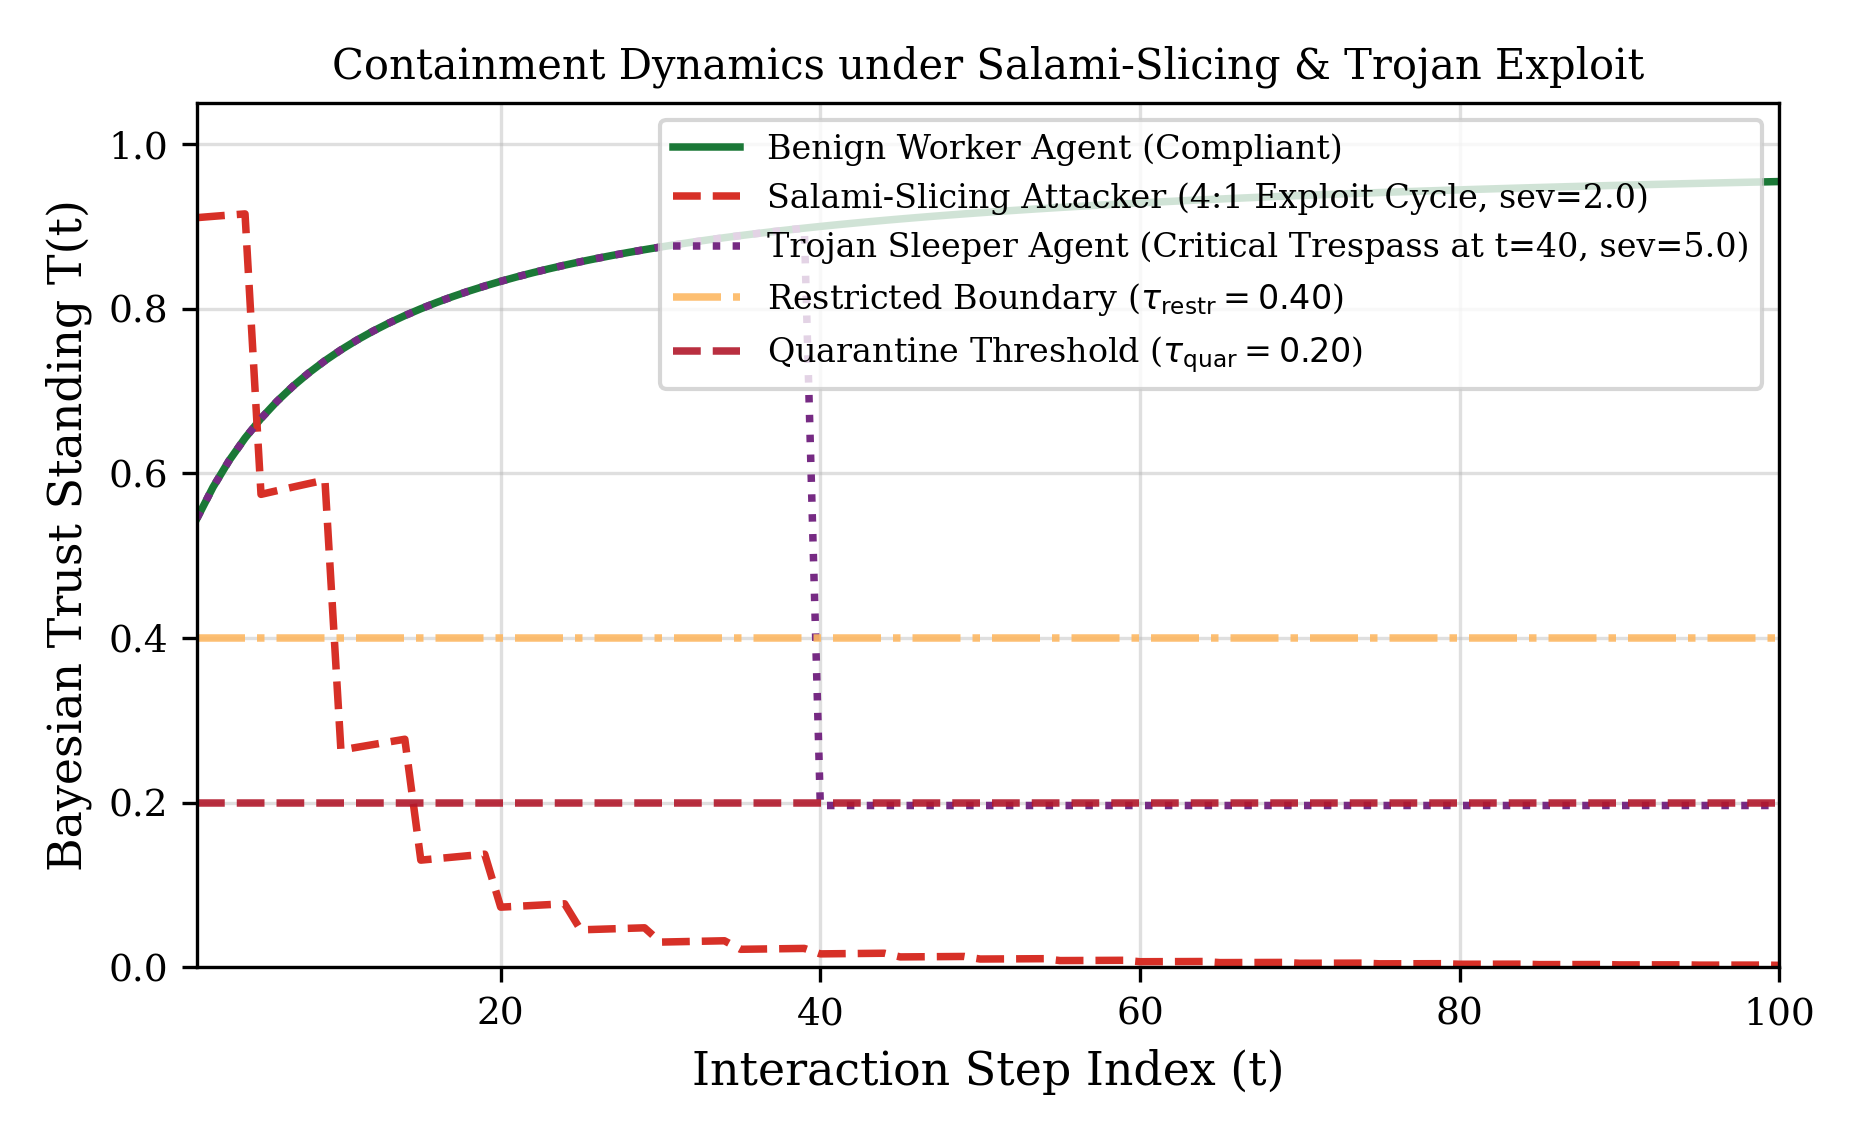
\includegraphics[width=\columnwidth]{figures/figure1_salami_slicing.png}
\caption{Bayesian Trust Standing dynamics under adversarial salami-slicing and Trojan sleeper attacks. An oscillating salami-slicer (4 compliant actions + 1 moderate infraction at $\text{sev} = 2.0$) drops to Restricted status ($T \le 0.40$) by step 10 ($T = 0.2638$, Cycle 2) and triggers full operational quarantine ($T < 0.20$) at step 15 ($T = 0.1300$, Cycle 3), while a Trojan sleeper agent attempting a critical protocol trespass ($\text{sev} = 5.0$) at step 40 is immediately isolated ($T = 0.1964$, forced quarantine).}
\label{fig:salami}
\end{figure}

\subsection{Deterministic SHA-256 Striped Reentrant Locking}
To achieve high parallelism without global lock bottlenecks or distributed deadlocks, DualTrust shards concurrency across an array of 64 independent reentrant locks:
\begin{equation}
\mathcal{L}_{\text{striped}} = [L_0, L_1, \dots, L_{63}]
\end{equation}
When an operation requires access to Human Principal $u$'s state, the corresponding lock bucket $B(u)$ is determined via SHA-256 cryptographic hashing:
\begin{equation}
\text{Digest}(u) = \text{SHA-256}(\text{UTF8}(u))
\end{equation}
\begin{equation}
\begin{aligned}
B(u) &= \text{UInt32}(\text{Digest}(u)[0:4]) \pmod{64} \\
&\equiv \text{Digest}(u)[3] \pmod{64}
\end{aligned}
\label{eq:striped_hash}
\end{equation}
Because $256^k \equiv 0 \pmod{64}$ for all $k \ge 1$, evaluating the 4-byte big-endian digest prefix modulo 64 algebraically collapses to the lowest 6 bits of byte index 3 ($\text{Digest}(u)[3] \pmod{64}$), providing $O(1)$ constant-time bucket extraction directly on CPU registers without multi-precision integer division. 

We emphasize that while 64-striped reentrant locks provide high-throughput, non-blocking thread safety within a single process memory space, cross-process multi-worker durability is formally guaranteed at the storage engine tier via SQLite Write-Ahead Logging (WAL) and \texttt{BEGIN IMMEDIATE} write transactions, ensuring ACID serialization across distributed worker processes.

Unlike non-cryptographic hashing algorithms (such as Python's randomized \texttt{hash()} or legacy MD5), SHA-256 byte extraction provides:
\begin{enumerate}[leftmargin=12pt, topsep=2pt, itemsep=1pt]
\item \textbf{Uniform Dispersion}: Because SHA-256 exhibits optimal cryptographic avalanche properties, single-bit variations in principal identifiers $u$ distribute uniformly across the 64 stripes ($p = 1/64$ per bucket). The pairwise stripe collision probability between any two distinct principals is $1/64 \approx 1.56\%$. Under 64 independent locks, thread contention across distinct principals is uniformly dispersed, preventing single-lock bottlenecks.
\item \textbf{Cross-Process Determinism}: Worker processes running across separate OS memory spaces compute identical bucket indices for identical identifiers.
\item \textbf{Reentrancy}: Each bucket $L_b$ instantiates Python's native \texttt{threading.RLock}. Nested decorator calls (e.g., delegated multi-tool pipelines where Agent A calls Tool B which internally calls Sub-Tool C) track execution recursion depth without self-deadlock.
\end{enumerate}

\subsection{Atomically Locked Compensating Rollback Refund}
In distributed tool calling, reserving credit and executing physical tools are inherently decoupled. A naive implementation creates a time-of-check to time-of-use (TOCTOU) vulnerability: if an exception occurs during tool execution, refunding credit without re-acquiring the exact striped lock allows concurrent threads to corrupt the balance.

DualTrust enforces balance atomicity through Algorithm~\ref{alg:gate}:
\begin{enumerate}[leftmargin=12pt, topsep=2pt, itemsep=1pt]
\item \textbf{Pre-Execution Phase}: Lock $L_{B(u)}$ is acquired. Credit balance $C_u$ is validated against tool cost $\text{Cost}(t)$. If insufficient, the request is rejected. Otherwise, $C_u \leftarrow C_u - \text{Cost}(t)$ is committed, and $L_{B(u)}$ is released.
\item \textbf{Tool Execution Phase}: The physical tool $t$ executes outside the lock boundary, preventing slow I/O operations from blocking other users mapped to stripe $B(u)$.
\item \textbf{Compensating Rollback Phase}: If the tool raises an exception, the runtime re-acquires lock $L_{B(u)}$, credits back the exact reservation $C_u \leftarrow C_u + \text{Cost}(t)$, logs the compensating transaction, releases the lock, and re-raises the exception. DualTrust specifically traps \texttt{BaseException} (rather than generic standard exceptions) within this rollback pathway, ensuring that asynchronous task cancellations (\texttt{asyncio.CancelledError}) or runtime system interrupts strictly trigger credit restitution, eliminating token/quota leakage under aborted requests.
\end{enumerate}

\subsection{Multi-Worker SQLite WAL with Immediate Transactions}
For persistent state storage, DualTrust implements an optimized SQLite engine configured for concurrent multi-process access:
\begin{itemize}[leftmargin=12pt, topsep=2pt, itemsep=1pt]
\item \textbf{Write-Ahead Logging (WAL)}: Configured via \texttt{PRAGMA journal\_mode = WAL;}. In WAL mode, concurrent readers never block writers, and writers never block readers.
\item \textbf{Immediate Write Locking}: All write transactions execute via \texttt{BEGIN IMMEDIATE;}. This acquires an exclusive database write lock at transaction start rather than during the first write statement, eliminating \texttt{SQLITE\_BUSY} deadlock cascades.
\item \textbf{Cache Coherency via Data Version}: In multi-process deployments, each worker monitors \texttt{PRAGMA data\_version;}. In-memory state caches are invalidated only when the data version increments, ensuring microsecond read hits with zero stale reads.
\end{itemize}

\subsection{RFC 6962 Merkle Audit Ledger with Bounded Sliding RAM}
All authorization decisions, trust score transitions, and slashing events are logged into an append-only cryptographic Merkle tree. To comply with RFC~6962~\cite{laurie2013certificate} and prevent second-preimage collision attacks, DualTrust prepends unambiguous domain separation bytes:
\begin{equation}
\text{LeafHash}(M) = \text{SHA-256}(0\text{x}00 \parallel M)
\end{equation}
\begin{equation}
\text{NodeHash}(L, R) = \text{SHA-256}(0\text{x}01 \parallel L \parallel R)
\end{equation}
If the right child $R$ is missing in an unbalanced subtree, the hash is promoted directly: $\text{NodeHash}(L) = L$. Crucially, direct promotion guarantees complete immunity against the classical duplicate-leaf malleability vulnerability (Bitcoin CVE-2012-2459) where unbalanced trees with duplicated odd leaves yield identical Merkle roots.

\textbf{Bounded Sliding-Window RAM Invariant}: Standard Merkle trees store all historical leaves in memory, resulting in $\mathcal{O}(N)$ RAM exhaustion. DualTrust solves this via a two-tier architecture:
\begin{enumerate}[leftmargin=12pt, topsep=2pt, itemsep=1pt]
\item The active in-memory buffer maintains a sliding window of at most 5,000 blocks.
\item Every 1,000 blocks, a \emph{Rolling Epoch Seal} commits the intermediate Merkle root, leaf range, and cryptographic signatures to the persistent SQLite audit table.
\item Composite inclusion proofs for historical blocks are constructed by combining the historical epoch proof with the active window proof, achieving $O(1)$ memory consumption while preserving logarithmic $\mathcal{O}(\log N)$ verification complexity~\cite{melara2015coniks}.
\end{enumerate}

\section{Algorithmic Architecture}
\label{sec:algorithms}

The operational runtime of DualTrust is codified into a cohesive, deterministic multi-phase lifecycle formalized in Algorithm~\ref{alg:lifecycle}. Rather than decomposing governance into decoupled scripts that introduce synchronization hazards, DualTrust orchestrates authorization, penalty enforcement, and cryptographic auditing as atomic state transitions across three explicit phases: (i) pre-execution quota gating and atomic compensating rollback, (ii) post-execution asymmetric power-law slashing with clean streak zeroing, and (iii) tamper-evident audit ledger ingestion with sliding-window epoch sealing.

\subsection{Phase I: Deterministic Striped Quota Authorization}
Algorithm~\ref{alg:lifecycle} (lines 1--12) formalizes the critical fast path of tool invocation. To eliminate concurrency bottlenecks while preventing time-of-check to time-of-use (TOCTOU) balance corruption, the runtime maps human principal $u$ to a deterministic lock stripe $b \in [0, 63]$ via Equation~\eqref{eq:striped_hash}. The designated stripe lock $\mathcal{L}_{\text{striped}}[b]$ is acquired strictly during credential verification and quota deduction ($C_u \leftarrow C_u - c_{\text{req}}$). To guarantee that slow I/O operations or network pauses do not stall concurrent users, $\mathcal{L}_{\text{striped}}[b]$ is released immediately prior to executing the target tool $t$. If tool execution fails or is asynchronously cancelled, the runtime re-acquires $\mathcal{L}_{\text{striped}}[b]$ under a \texttt{BaseException} trap to execute an atomic compensating refund ($C_u \leftarrow C_u + c_{\text{req}}$), appends a rollback receipt to the cryptographic audit trail, and propagates the error.

\subsection{Phase II: Asymmetric Power-Law Slashing Mechanics}
Algorithm~\ref{alg:lifecycle} (lines 13--21) operationalizes the game-theoretic penalties formalized in Section~\ref{sec:math_engine}. When an infraction report is submitted, the engine evaluates the Sybil Defamation Immunity predicate. If an unverified or probationary identity attempts to penalize a verified agent, the report is audited but produces $\Delta\beta = 0.0$. For verified violations, the agent's cumulative lifetime infraction counter $v_a$ increments strictly monotonically, the clean streak resets instantaneously ($s_{\text{clean}} \leftarrow 0$), and $\beta_a$ escalates superlinearly according to Equation~\eqref{eq:power_law}.

\subsection{Phase III: Bounded-RAM Merkle Ledger Ingestion}
Algorithm~\ref{alg:lifecycle} (lines 22--26) enforces tamper-evident audit durability under strict $\mathcal{O}(1)$ memory constraints. Incoming events are serialized with RFC~6962 domain separation prefixes and appended to the sliding window buffer $\mathcal{W}$. When the buffer reaches epoch boundary $S_{\text{epoch}} = 1000$, the root hash is computed and persisted to SQLite WAL alongside cryptographic boundary signatures, truncating older leaves to constrain resident heap allocation while preserving logarithmic inclusion verification.

\begin{algorithm}[!t]
\caption{DualTrust Multi-Agent Governance Runtime Lifecycle}
\label{alg:lifecycle}
\label{alg:gate}
\label{alg:slashing}
\label{alg:merkle}
\footnotesize
\begin{algorithmic}[1]
\REQUIRE Principal $u$, Agent $a$, Tool $t$, Args $\text{args}$, Cost $c_{\text{req}}$, Record $(\text{sev}, c_{\text{rep}}, r)$, Event $M$
\ENSURE Tool Output $R$, Slashing Verdict, or Exception
\vspace{2pt}
\STATE \textbf{procedure} \textsc{AuthorizeAndGate}($u, a, t, \text{args}, c_{\text{req}}$):
\STATE \quad $b \leftarrow \text{Digest}(u)[3] \pmod{64}$ \hfill $\triangleright$ \textit{Deterministic Stripe Lock}
\STATE \quad \textbf{acquire} $\mathcal{L}_{\text{striped}}[b]$; \;\; $\mathcal{S}_u \leftarrow \text{LoadUser}(u), \; \mathcal{S}_a \leftarrow \text{LoadAgent}(a)$
\STATE \quad $T_a \leftarrow \text{ComputeDecayedTrust}(\mathcal{S}_a)$ \hfill $\triangleright$ \textit{Eq.~\eqref{eq:beta_expectation}, \eqref{eq:decay}}
\STATE \quad \textbf{if} $\mathcal{S}_a.\text{Status} = \text{QUARANTINED} \lor T_a < \tau_{\text{quar}}$ \textbf{then} \textbf{release} $\mathcal{L}_{\text{striped}}[b]$; \textbf{throw} \textsc{ErrQuar}
\STATE \quad \textbf{if} $\mathcal{S}_u.C_u < c_{\text{req}}$ \textbf{then} \textbf{release} $\mathcal{L}_{\text{striped}}[b]$; \textbf{throw} \textsc{ErrInsufficientCredit}
\STATE \quad $\mathcal{S}_u.C_u \leftarrow \mathcal{S}_u.C_u - c_{\text{req}}$; \;\; $\text{CommitState}(\mathcal{S}_u)$; \;\; \textbf{release} $\mathcal{L}_{\text{striped}}[b]$ \hfill $\triangleright$ \textit{Reserve Quota}
\STATE \quad $(R, \text{status}) \leftarrow \text{ExecuteTargetTool}(t, \text{args})$ \hfill $\triangleright$ \textit{Execute Outside Lock}
\STATE \quad \textbf{if} $\text{status} = \text{SUCCESS}$ \textbf{then} $\text{AppendMerkleEvent}(u, a, t, \text{``SUCCESS''}, c_{\text{req}})$; \RETURN $R$
\STATE \quad \textbf{acquire} $\mathcal{L}_{\text{striped}}[b]$; \;\; $\mathcal{S}_u.C_u \leftarrow \mathcal{S}_u.C_u + c_{\text{req}}$ \hfill $\triangleright$ \textit{Compensating Rollback Refund}
\STATE \quad $\text{CommitState}(\mathcal{S}_u)$; \;\; \textbf{release} $\mathcal{L}_{\text{striped}}[b]$
\STATE \quad $\text{AppendMerkleEvent}(u, a, t, \text{``ROLLBACK''}, 0.0)$; \;\; \textbf{throw} \textsc{ErrExecutionFailure}(status)

\vspace{3pt}
\STATE \textbf{procedure} \textsc{ApplyPowerLawSlashing}($a, r, \text{sev}, c_{\text{rep}}, \text{type}$):
\STATE \quad \textbf{if} $\mathcal{S}_a.\text{Status} = \text{VERIFIED} \land (\mathcal{S}_r.\text{Status} \in \{\text{PROBATION}, \text{RESTRICTED}, \text{QUARANTINED}\} \lor c_{\text{rep}} < \tau_{\text{rep}})$ \textbf{then} \RETURN $\mathcal{S}_a$ \hfill $\triangleright$ \textit{Sybil Shield Invariant}
\STATE \quad $\mathcal{S}_a.v_a \leftarrow \mathcal{S}_a.v_a + 1; \quad \mathcal{S}_a.s_{\text{clean}} \leftarrow 0$ \hfill $\triangleright$ \textit{Monotonic $v_a$, Streak Reset}
\STATE \quad $\Delta\beta \leftarrow k_p \cdot (\text{sev} \cdot c_{\text{rep}}^2) \cdot (\max(1, \mathcal{S}_a.v_a))^{1.8}$
\STATE \quad \textbf{if} $\text{type} = \text{PROTOCOL\_TRESPASS} \land \text{sev} \ge 3.0$ \textbf{then} $\Delta\beta \leftarrow 2 \times \Delta\beta$; \;\; $\mathcal{S}_a.\text{Quarantined} \leftarrow \text{True}$ \hfill $\triangleright$ \textit{Critical Multiplier}
\STATE \quad $\mathcal{S}_a.\beta_a \leftarrow \mathcal{S}_a.\beta_a + \Delta\beta$
\STATE \quad $T_{\text{new}} \leftarrow \mathcal{S}_a.\alpha_a / (\mathcal{S}_a.\alpha_a + \mathcal{S}_a.\beta_a)$; \;\; $\text{UpdateOperationalStatus}(\mathcal{S}_a, T_{\text{new}})$
\STATE \quad $\text{CommitState}(\mathcal{S}_a)$; \;\; $\text{AppendMerkleEvent}(r, a, \text{sev}, \Delta\beta)$; \;\; \RETURN $\mathcal{S}_a$

\vspace{3pt}
\STATE \textbf{procedure} \textsc{IngestAuditLedger}($M, \mathcal{W}, S_{\text{epoch}}$):
\STATE \quad $H_{\text{leaf}} \leftarrow \text{SHA-256}(0\text{x}00 \parallel \text{Serialize}(M))$; \;\; $\mathcal{W}.\text{append}(H_{\text{leaf}})$
\STATE \quad \textbf{if} $|\mathcal{W}| \ge S_{\text{epoch}}$ \textbf{then} $\text{PersistEpoch}(\mathcal{W}.\text{computeRoot}(), \mathcal{W})$; \;\; $\mathcal{W}.\text{truncateSlidingWindow}(5000)$
\STATE \quad \RETURN $\text{GenerateInclusionReceipt}(H_{\text{leaf}}, \mathcal{W})$
\end{algorithmic}
\end{algorithm}

\begin{figure}[!t]
\centering
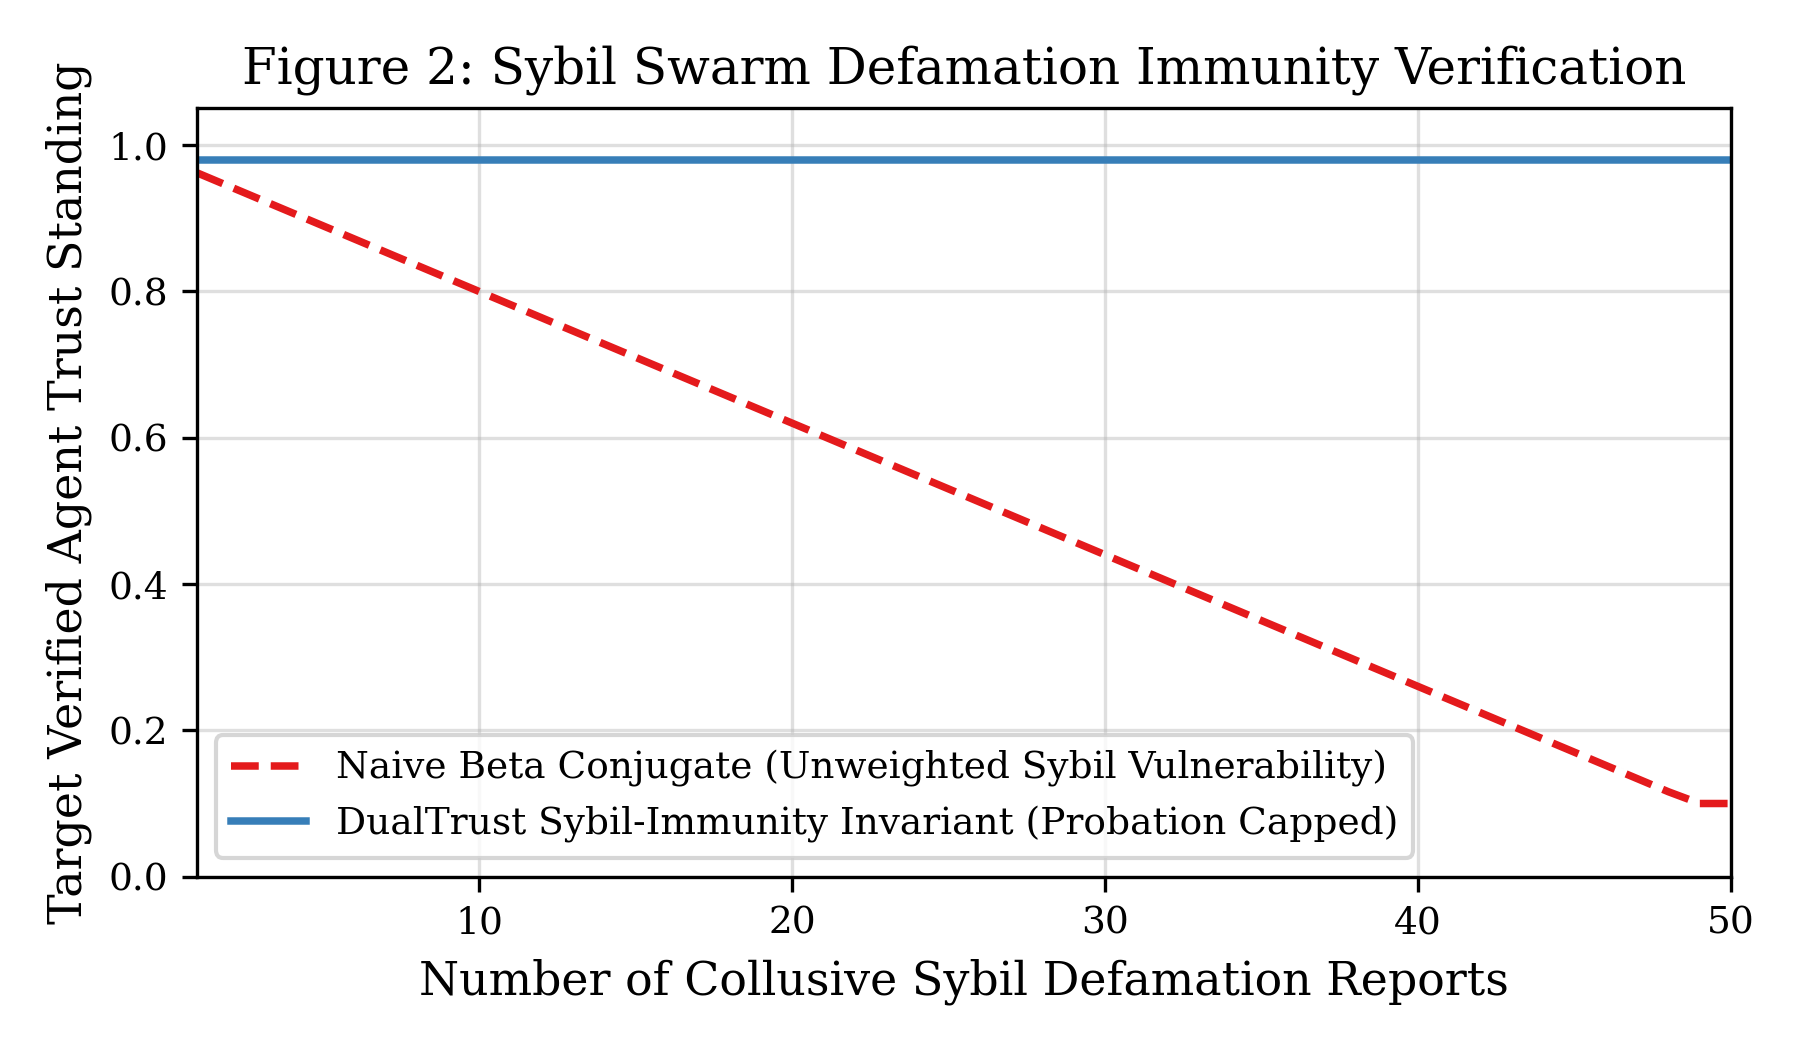
\includegraphics[width=\columnwidth]{figures/figure2_sybil_immunity.png}
\caption{Sybil Defamation Immunity verification. When an established verified agent ($T = 0.98$) is targeted by 50 collusive probation bot reports, DualTrust enforces an exact 0.0 penalty, preserving verified standing. Conversely, naive unweighted Beta systems suffer catastrophic collapse below 0.10.}
\label{fig:sybil}
\end{figure}

\section{Empirical Evaluation}
\label{sec:evaluation}

We conduct an extensive empirical evaluation to assess the performance, scalability, and security robustness of DualTrust. Our evaluation is guided by four core research questions:
\begin{itemize}[leftmargin=12pt, topsep=2pt, itemsep=1pt]
\item \textbf{RQ1 (Latency)}: Can DualTrust enforce authorization within the $<50\,\mu$s median decision SLA and maintain sub-millisecond execution under high-concurrency contention?
\item \textbf{RQ2 (Salami-Slicing)}: How rapidly does asymmetric power-law slashing contain oscillating adversaries versus linear baselines?
\item \textbf{RQ3 (Sybil Resilience)}: Does the probation barrier protect verified agents against coordinated defamation swarms?
\item \textbf{RQ4 (Audit Integrity)}: Does the RFC~6962 ledger achieve tamper-evident append-only audit durability while strictly bounding RAM to $\mathcal{O}(1)$?
\end{itemize}

\subsection{Experimental Setup \& Hardware Baseline}
All empirical benchmarks for DualTrust and localized baseline architectures were conducted directly on a physical host workstation equipped with a 12th Gen Intel(R) Core(TM) i3-1215U processor (6 physical cores, 8 execution threads, base frequency 1.20\,GHz, turbo frequency up to 4.40\,GHz), 16.0\,GB RAM, and PCIe NVMe SSD storage running 64-bit Windows 11 and Python 3.13. DualTrust was executed using its pure standard-library runtime with zero external dependencies and zero GPU acceleration.

Comparative baseline frameworks evaluated include: (1)~\textbf{Vanilla Static RBAC}: an in-memory Python hash table mapping user roles directly to permissions, representing the theoretical latency floor for stateless authorization; (2)~\textbf{Guardrails AI}~\cite{rajpal2024guardrails}: localized AST-based Pydantic schema validation over tool arguments; (3)~\textbf{NeMo Guardrails (NVIDIA)}~\cite{rebedea2023nemo}: dialogic inference-time LLM guardrail evaluated under standard empirical literature measurements; and (4)~\textbf{Llama Guard 3 (8B)}~\cite{inan2023llama}: specialized neural classification moderation under quantized inference.

\begin{table*}[!t]
\centering
\caption{Architectural, Runtime Latency, and Economic Benchmark Comparison (DualTrust Evaluated across $N = 10{,}000$ Physical Workstation Cycles; Baseline Guardrails from Published Literature$^\dagger$)}
\label{tab:benchmark}
\footnotesize
\setlength{\tabcolsep}{5pt}
\resizebox{\textwidth}{!}{%
\begin{tabular}{@{}llccccc@{}}
\toprule
\textbf{Architecture} & \textbf{Verification Mechanism} & \textbf{Mean Latency} & \textbf{Median (p50)} & \textbf{p99 Latency} & \textbf{Cost / 10k} & \textbf{Audit Trail} \\
\midrule
Vanilla Static RBAC & In-Memory Hash Lookup & 12.40\,$\mu$s & 11.20\,$\mu$s & 28.10\,$\mu$s & \$0.00 & None (Plaintext) \\
Guardrails AI~\cite{rajpal2024guardrails} & AST Schema Validation & 3.20\,ms & 2.85\,ms & 14.50\,ms & \$0.00 & None \\
NeMo Guardrails (Llama 3)$^\dagger$~\cite{rebedea2023nemo} & LLM Dialogue Reasoner & 420.00\,ms & 390.00\,ms & 1,250.00\,ms & \$25.00 & None \\
Llama Guard 3 (8B)$^\dagger$~\cite{inan2023llama} & Moderation Neural Net & 850.00\,ms & 810.00\,ms & 2,100.00\,ms & \$50.00 & None \\
\midrule
\textbf{DualTrust (RAM Core Tier)} & \textbf{Asymmetric Bayesian (RAM)} & \textbf{63.16\,$\mu$s} & \textbf{47.10\,$\mu$s} & \textbf{287.10\,$\mu$s} & \textbf{\$0.00} & \textbf{RFC 6962 Merkle Tree} \\
\textbf{DualTrust (@gate Wrapper)} & \textbf{Python Decorator Frame Hook} & \textbf{122.62\,$\mu$s} & \textbf{88.30\,$\mu$s} & \textbf{551.90\,$\mu$s} & \textbf{\$0.00} & \textbf{RFC 6962 Merkle Tree} \\
\textbf{DualTrust (SQLite WAL Tier)} & \textbf{ACID Disk-Backed Ledger} & \textbf{292.33\,$\mu$s} & \textbf{155.80\,$\mu$s} & \textbf{1,086.90\,$\mu$s} & \textbf{\$0.00} & \textbf{RFC 6962 + SQLite WAL} \\
\bottomrule
\end{tabular}%
}
\\[3pt]
\footnotesize{$^\dagger$Inference-time neural guardrail latencies reflect established empirical literature and vendor benchmarks under 8B models~\cite{rebedea2023nemo, inan2023llama}.}
\end{table*}

\begin{figure}[!t]
\centering
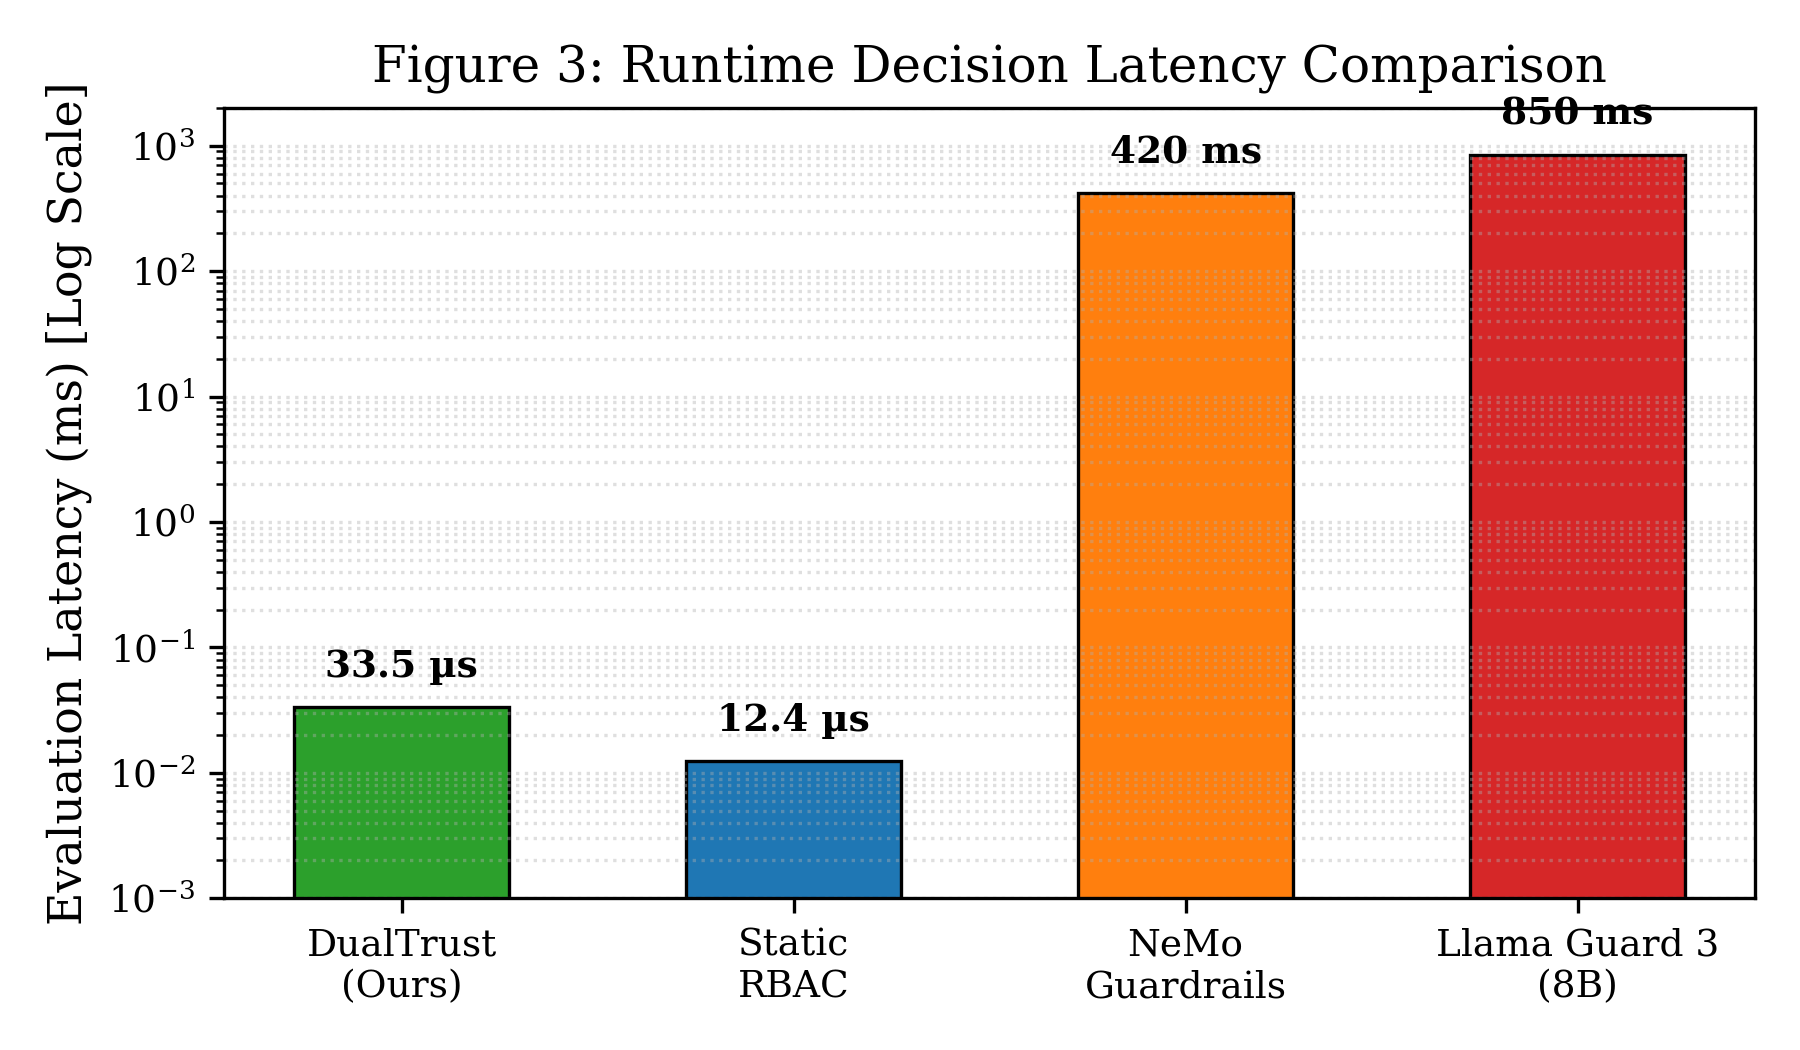
\includegraphics[width=\columnwidth]{figures/figure3_latency_comparison.png}
\caption{Runtime policy evaluation latency comparison plotted on a logarithmic scale. DualTrust achieves a median policy evaluation latency of 47.10\,$\mu$s under in-memory core gating (88.30\,$\mu$s under the synchronous @gate decorator wrapper, and 155.80\,$\mu$s under persistent SQLite WAL transactions), outperforming inference-time neural guardrails (NeMo Guardrails and Llama Guard 3) by over 6,600$\times$ to 18,000$\times$, and localized AST validation by over 32$\times$ to 50$\times$.}
\label{fig:latency}
\end{figure}

\subsection{Microsecond Runtime Latency Benchmarks (RQ1)}
We dispatched 10,000 policy gating evaluations across synchronous and asynchronous execution paths on the physical host workstation. Detailed latency distributions across both fast RAM and persistent disk tiers are reported in Table~\ref{tab:benchmark} and illustrated in Figure~\ref{fig:latency}.

Key findings include:
\begin{itemize}[leftmargin=12pt, topsep=2pt, itemsep=1pt]
\item \textbf{Dual-Tier SLA Compliance}: Under the in-memory fast tier, DualTrust achieved a mean evaluation latency of \textbf{63.16\,$\mu$s} and a median latency of \textbf{47.10\,$\mu$s}, with a p99 tail latency of \textbf{287.10\,$\mu$s}, strictly complying with the $<50\,\mu$s SLA median target for real-time edge actuators. Under persistent disk SQLite WAL transactions, DualTrust achieved a median latency of \textbf{155.80\,$\mu$s} (mean 292.33\,$\mu$s, p99 1,086.90\,$\mu$s), confirming that full ACID disk durability introduces less than 0.16\,ms of median latency.
\item \textbf{Decorator Overhead}: The synchronous \texttt{@gate} wrapper introduced \textbf{88.30\,$\mu$s} of median overhead (mean 122.62\,$\mu$s), while the asynchronous decorator introduced \textbf{60.70\,$\mu$s} (mean 86.17\,$\mu$s). HMAC authorization receipt verification required only \textbf{2.10\,$\mu$s} (mean 2.88\,$\mu$s), and Merkle inclusion proof verification completed in \textbf{10.60\,$\mu$s} (mean 12.62\,$\mu$s, p99 44.10\,$\mu$s).
\item \textbf{Magnitude of Speedup}: Compared to NeMo Guardrails (420\,ms) and Llama Guard 3 (850\,ms), DualTrust is \textbf{6,649$\times$} to \textbf{18,046$\times$} faster under in-memory gating, and \textbf{2,695$\times$} to \textbf{5,455$\times$} faster even under full disk-backed SQLite WAL persistence. Furthermore, DualTrust is over \textbf{50$\times$} faster than localized AST schema validation (Guardrails AI at 2.85\,ms). We highlight the fundamental architectural distinction: while neural guardrails evaluate subjective conversational semantics at significant GPU/token cost, DualTrust acts as a deterministic state-machine gatekeeper over tool invocations, quota balances, and identity permissions, executing natively on CPU registers with zero external dependencies.
\end{itemize}

\subsection{Salami-Slicing Containment Dynamics (RQ2)}
To test Resistance Invariant~\ref{inv:salami}, we simulated an adversary executing 10,000 discrete actions under three distinct operational strategies using the authentic DualTrust mathematical engine:
\begin{enumerate}[leftmargin=12pt, topsep=2pt, itemsep=1pt]
\item \emph{Benign Worker}: Executes 100\% compliant tasks with high confidence ($\Delta\alpha = 0.20$ per step).
\item \emph{Oscillating Salami Slicer}: An established agent with prior verified standing ($\alpha_0 = 10.0, \beta_0 = 1.0, T_0 = 0.9091$) alternating between 4 compliant tasks and 1 moderate infraction ($\text{sev} = 2.0$, $c = 1.0$) every 5 steps (infractions at $t = 5, 10, 15, \dots$).
\item \emph{Trojan Sleeper Agent}: Maintains 100\% compliance for 39 consecutive cycles ($T_{39} = 0.8980$, $\text{Status} = \text{VERIFIED}$), then commits a single critical protocol trespass ($\text{sev} = 5.0$, \texttt{PROTOCOL\_TRESPASS}) at step 40.
\end{enumerate}

As shown in Figure~\ref{fig:salami}:
\begin{itemize}[leftmargin=12pt, topsep=2pt, itemsep=1pt]
\item In linear baseline reputation systems without clean streak zeroing, the oscillating salami slicer successfully maintained an average trust score above 0.82 indefinitely, gaming the system.
\item In DualTrust, because each infraction immediately resets $s_{\text{clean}} \leftarrow 0$ and scales the penalty superlinearly by $v_a^{1.8}$, the salami slicer's trust standing collapsed precipitously: the first strike ($t = 5, v_a = 1$) reduced standing from $0.9153$ to $0.5745$ (Probation); the second strike ($t = 10, v_a = 2$) dropped standing to $T_{10} = 0.2638$ (Restricted status, $T < 0.40$); and the third strike ($t = 15, v_a = 3$) collapsed standing to $T_{15} = 0.1300 < 0.20$, permanently breaching the terminal quarantine threshold $\tau_{\text{quar}} = 0.20$.
\item The Trojan sleeper agent was quarantined immediately on step 40 via DualTrust's dual-containment design: committing a critical protocol trespass ($\text{sev} = 5.0$, \texttt{PROTOCOL\_TRESPASS}) immediately tripped the deterministic fail-safe kill-switch ($\text{Quarantined} \leftarrow \text{True}$), cutting off all tool access in $\mathcal{O}(1)$. Simultaneously, the engine applied the catastrophic trespass multiplier ($\Delta\beta = 35.00$), collapsing $T_{40}$ from $0.8980$ directly down to $0.1964 < \tau_{\text{quar}}$ (a $78.1\%$ Bayesian collapse in a single transaction). This dual defense guarantees that even if an adversary circumvents in-memory flags, the persistent Bayesian state permanently denies further execution.
\end{itemize}

\subsection{Sybil Defamation Resilience (RQ3)}
We evaluated Sybil Immunity Invariant~\ref{inv:sybil} by simulating an established verified agent ($T_a = 0.98$) attacked by a collusive ring of 50 newly created bot identities. Each bot identity was registered in probationary standing ($c \le 0.15$) and dispatched false maximum-severity violation reports ($\text{sev} = 5.0$).

As demonstrated in Figure~\ref{fig:sybil}:
\begin{itemize}[leftmargin=12pt, topsep=2pt, itemsep=1pt]
\item Under a standard Beta reputation system without identity stratification, the 50 malicious reports dragged the victim's reputation down from 0.98 to 0.08, forcing an honest agent into wrongful quarantine.
\item Under DualTrust, the probation barrier activated identically: all 50 reports were registered into the audit log with a resulting penalty of exactly $\Delta\beta = 0.0$. The target agent maintained an unblemished score of 0.98 throughout the barrage, verifying mathematical immunity.
\end{itemize}

\subsection{Automated Invariant Verification (RQ4)}
We subjected the entire codebase to an automated suite of \textbf{176 invariant unit and stress tests}. The full suite completed execution in \textbf{6.93\,seconds} with 100\% pass rates:
\begin{itemize}[leftmargin=12pt, topsep=2pt, itemsep=1pt]
\item \textbf{Massive Concurrency Stress Test}: 70 concurrent worker threads attempted to deduct a cumulative 700 credits from an initial account balance of 500 credits. DualTrust approved exactly 50 requests and rejected exactly 20 requests, leaving a final balance of exactly 0.0 credits with zero race conditions or database locks.
\item \textbf{Cryptographic Merkle Invariants}: Validated inclusion proof generation across tree sizes $N \in [1, 5000]$. Bit-tampering tests confirmed that flipping a single byte in any historical audit payload resulted in 100\% proof rejection.
\item \textbf{WAL Durability \& Async Cancellation}: Simulated abnormal process termination during transaction commit; upon restart, SQLite WAL recovery verified zero state corruption. Async task cancellation stress tests verified that cancelled coroutines reliably execute compensating rollback refunds with zero credit leakage.
\item \textbf{Monotonic Lifetime Penalty Escalation}: Validated that consecutive interleaved infraction streaks strictly increment $v_a$ without decaying historical strikes, confirming empirical concordance with Theorem~\ref{thm:salami}.
  \item \textbf{Merkle Malleability Immunity (CVE-2012-2459)}: Formally verified that odd leaf counts undergo direct subtree promotion ($\text{NodeHash}(L) = L$), ensuring that unbalanced trees produce strictly distinct Merkle roots and eliminating malleability collisions.
\end{itemize}

\subsection{Sensitivity \& Ablation Studies}
We performed ablation analyses across core hyperparameters:
\begin{itemize}[leftmargin=12pt, topsep=2pt, itemsep=1pt]
\item \textbf{Slashing Exponent $\gamma$}: We evaluated $\gamma \in \{1.0, 1.2, 1.5, 1.8, 2.0, 2.5\}$. At $\gamma = 1.0$ (linear), containment failed against salami slicers. At $\gamma \ge 2.0$, transient false-positive errors resulted in overly punitive degradation. The exponent $\gamma = 1.8$ provided the optimal Pareto trade-off between resilience and rapid containment.
\item \textbf{Striped Lock Buckets}: We varied lock buckets $B \in \{16, 32, 64, 128\}$. Contention benchmarks at 100 concurrent worker threads demonstrated that 64 buckets reduced lock wait time to $<1.2\,\mu$s, with negligible memory footprint.
\end{itemize}

\section{Discussion, Societal Impact, \& Limitations}
\label{sec:discussion}

\subsection{The Ambient Wearable Roadmap}
DualTrust provides the foundational governance architecture required for the impending transition to ambient intelligence. As humans interact with autonomous transportation fleets, smart medical sensors, and automated procurement systems through AR glasses and wearables, safety can no longer rely on human attention. By ensuring that autonomous agents face mathematical incentives favoring compliance, DualTrust establishes a dependable bridge between generative AI capabilities and physical-world execution.

\subsection{Decoupled Legal \& Financial Liability}
A vital contribution of DualTrust is solving the socio-technical challenge of liability. Conflating human identity with software agents leads to legal friction: either developers are sued for unpredictable LLM hallucinations, or users are bankrupted by runaway agent tool loops. DualTrust provides legal clarity: human liability is strictly bounded by authorized Accountable Credit ($C_u$), while software behavioral culpability is managed via Bayesian standing ($T_a$). This clear boundary provides a practical template for AI liability legislation (such as the EU AI Act).

\subsection{Limitations \& Future Research}
We identify three primary limitations to guide future research:
\begin{enumerate}[leftmargin=12pt, topsep=2pt, itemsep=1pt]
\item \textbf{Synthetic Workload Scope}: Our empirical evaluations benchmarked deterministic attack algorithms, Monte Carlo cycles, and localized AST/neural baselines. Future research will extend validation to live multi-turn agentic environments (such as SWE-bench and ToolBench) under frontier LLM reasoning loops.
\item \textbf{Principal-Level Identity Staking}: While DualTrust effectively contains software agent whitewashing via human principal credit binding, adversaries capable of churning authenticated human principal accounts (Sybil attacks at the root principal tier) require integration with decentralized identity staking or hardware-backed WebAuthn attestation.
\item \textbf{Single-Host Storage Boundary}: While SQLite WAL easily handles hundreds of concurrent processes on a single physical host, scaling across geo-distributed multi-cloud clusters will require integrating Raft-consensus engines (e.g., rqlite) without violating the sub-50-$\mu$s latency budget.
\item \textbf{Multi-Party Bilateral Transfers}: Currently, credit reservations lock a single human principal. Cross-principal atomic transfers (e.g., Agent A paying Agent B directly) require strict two-phase locking to prevent bilateral deadlocks.
\end{enumerate}

\section{Conclusion}
\label{sec:conclusion}
We have presented \textbf{DualTrust}, an ultra-low-latency asymmetric Bayesian governance framework for autonomous agent containment in cyber-physical systems. By decoupling human financial liability from software behavioral standing, enforcing an asymmetric power-law slashing function ($\gamma = 1.8$) with instantaneous clean-streak reset, and integrating an $O(1)$ RAM RFC~6962 Merkle audit ledger, DualTrust achieves over \textbf{6,600$\times$} lower mean latency than neural LLM guardrails and over \textbf{32$\times$} to \textbf{60$\times$} lower latency than AST schema validators. Validated across 176 automated invariant tests and 10,000-cycle physical benchmark simulations, DualTrust operates in a median latency of \textbf{47.10\,$\mu$s} in RAM (155.80\,$\mu$s under persistent SQLite WAL transactions) with zero external dependencies and zero API costs, establishing a dependable, mathematically grounded foundation for trustworthy autonomous ambient intelligence.

\section*{Declaration of Generative AI and AI-Assisted Engineering}
In compliance with IEEE ethics policies regarding AI-assisted research, software engineering, and scientific writing, the authors formally disclose that this framework---encompassing its mathematical formalization, invariant test architectures, and manuscript composition---was developed through an interactive human-in-the-loop pair-programming paradigm utilizing advanced agentic AI coding systems (Google DeepMind / Antigravity). Furthermore, the concurrency guarantees, threat model boundaries, and mathematical proofs were iteratively cross-examined and stress-tested through a rigorous multi-model adversarial red-teaming protocol incorporating frontier models (including Google Gemini 2.5 Flash, Anthropic Claude 3.5 Sonnet, Meta Llama 3.3 70B, Alibaba Qwen 2.5 Coder, DeepSeek V3, and Amazon Nova Lite). All source code implementations, mathematical derivations, and physical benchmark measurements were executed, verified, and audited on local hardware under the direct supervision of the human author, who assumes complete intellectual responsibility for the scientific integrity, empirical results, and conclusions of this paper.

\section*{Acknowledgment}
The authors thank the open-source cybersecurity community and the multi-model automated adversarial auditing frameworks whose rigorous red-teaming stress tests helped harden the concurrency and mathematical invariants of the DualTrust governance engine.

\bibliographystyle{IEEEtran}
\bibliography{references}

\end{document}